\title{Solar radiation, environmental temperature, and warm-up curve}
\date{}

\documentclass[12pt]{article}
\usepackage{amsmath}
\usepackage{mathabx}
\usepackage{graphics}
\usepackage[top=1in, bottom=1in, left=1in, right=1in]{geometry}
\usepackage{tabu}
\usepackage[english]{babel}
\usepackage{natbib}
\bibliographystyle{evolution}
\usepackage{rotating}
\usepackage[capitalize, sort&compress]{cleveref}


% Tell latex how it can introduce linebreaks if necessary.
\hyphenation{Bar-thol-o-mew}

\begin{document}
\maketitle
Here, we describe adapted models for temporal changes in solar radiation and environmental temperature, and changes in body temperature during warm-up phase for our purpose.
%First, we model changes in solar radiation as function of latitude, day of the year, and time of the day.
%Second, we use solar radiation to model change in daily temperature.
%Third, we use the two components above and thermodynamic principles to model the warm-up phase of both endothermic and ectothermic insects.
Most of the equations are derived from \citet{Campbell2012}. 
However, rather than going into technical details of the numerous factors that influences the three quantities above, we greatly simplify model. 
Thus, we only keep the main factors in order to reproduce general patterns. 

\section*{Solar radiation: SR}
As in \citet{Campbell2012}, we model zenith angle ($\psi$) at time $t$ as
\begin{equation}  \label{eq:psi}
\cos(\psi) = \sin(\phi) \sin(\delta) + \cos(\phi) \cos(\delta) \cos[15 (t- t_0)] 
\end{equation}
Here, $\phi$ denotes latitude, $\delta$ denotes solar declination which varies between 23.45$^\circ$ and  -23.45$^\circ$ at summer and winter solstice 
($\delta$ as in equation 11.2 in \citet{Campbell2012} and only depends of the day of the year). 
$t_0$ represents the time of solar noon and since we do not span across longitude, we fix $t_0 = 12$.
For simplicity, we assume that solar radiation is \[SR = S_0 \cos(\psi) \] where $S_0 = 1361 \mbox{W.m}^{-2}$. 
\cref{fig:rad} shows variations of SR at different latitudes during solstice and equinox.

\begin{figure}
\begin{center}
	\scalebox{0.75}{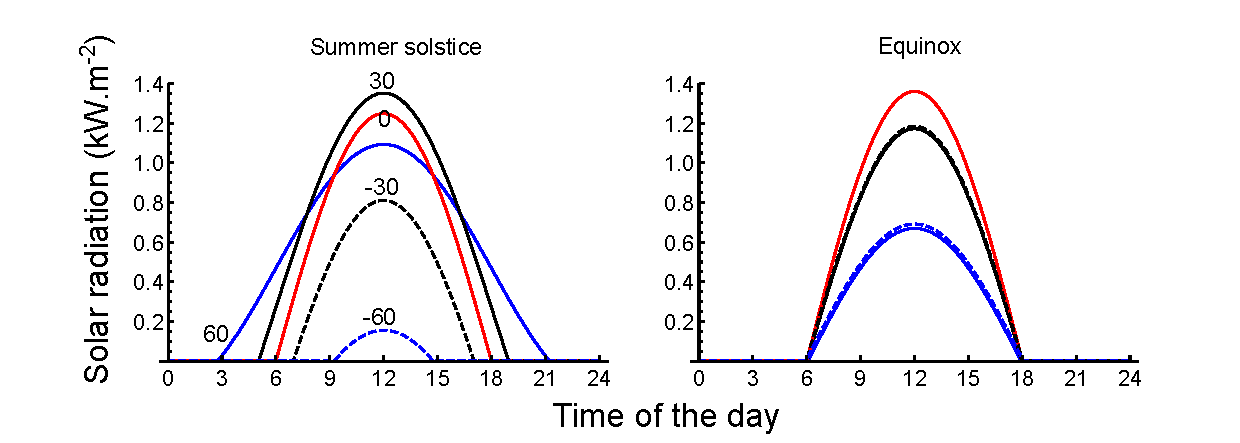
\includegraphics{fig1}}
	\caption{Change in solar radiation during the course of the day at different latitudes---color coded and labeled numbers. 
	Northern latitudes are denoted by positive numbers.  
	}
	\label{fig:rad}
\end{center}
\end{figure}

\section*{Environmental temperature: $T_e$}
We define environmental temperature as the `real' temperature and thus mean air temperature including the effect of humidity, wind speed, and so on. 
Change in environmental temperature depends on solar radiation and surface emissivity of the earth.
$T_e(t)$ (in $^\circ$C) is the solution of the following differential equation
\[
	\frac{dT_e}{dt} = r_1 SR(t)  - r_2 \sigma  \varepsilon (T_e(t)+ 273.2)^4
\]
Before sunset and after sunrise SR = 0,  $T_e(0)$ is free parameter and is the environmental temperature at midnight. 
$\sigma$ is Stefan-Boltzman constant.
The coefficients $r_1$ and $r_2$ are free parameters used to shape temperature changes.
With imagination, they can account for the effects of humidity, cloud cover, wind and so on.
For our purpose, we show different changes in daily temperature by tuning $r_1$ and $r_2$ (\cref{fig:temp}).


\begin{figure}
\begin{center}
	\scalebox{0.75}{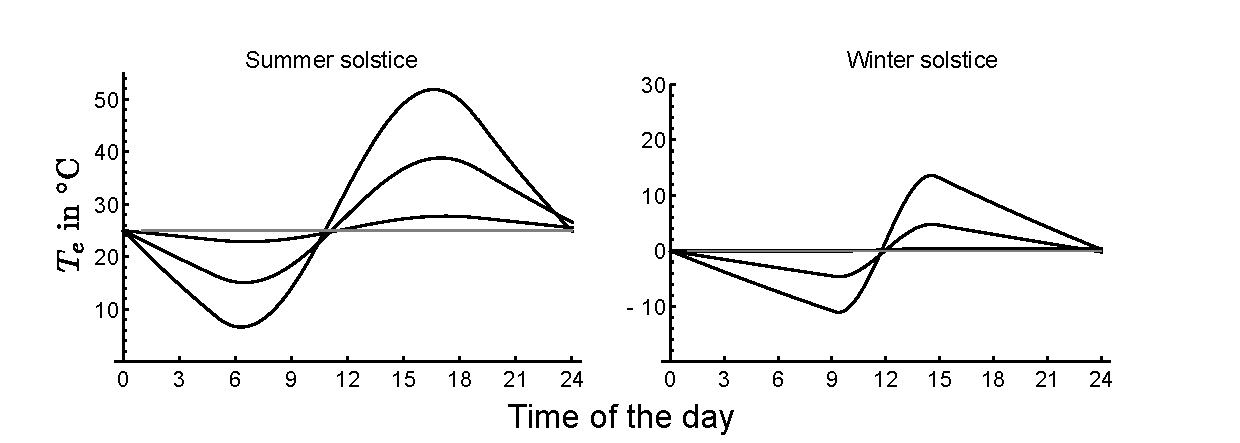
\includegraphics{fig2}}
	\caption{Fluctuation in environmental temperature at 30$^\circ$ N during summer solstice (left) and at 60$^\circ$ N during winter solstice (right).
	The different amplitude are obtained by tuning $r_1$ and $r_2$. 
	For left panel and from large to small fluctuation $r_1 = 8 , r_2 = 0.00825$, $r_1 = 4 , r_2 = 0.004125$, and $r_1 = 0.8 , r_2 = 0.000825$.
	For right panel and  from large to small fluctuation, $r_1 = 52 , r_2 = 0.004125$, $r_1 = 20 , r_2 = 0.00165$, and $r_1 = 0.8 , r_2 =1.1 \times 10^{-5}$.
	The gray line shows initial temperature at $t = 0$.
	}
	\label{fig:temp}
\end{center}
\end{figure}

\section*{Change in thoracic temperature: $T_{th}$}
We describe temperature change in two parts of the body (thorax and the rest-of-the-body) as a function of solar radiation and environmental temperature during warm-up (for ecothermic and endothermic). 
The main variable is the thoracic temperature $T_{th}$ because the individual cannot forage unless $T_{th} > T_w$ where
\begin{equation} \label{eq:Tw}
	T_w(z_{th}) = c_0+ c_1 z_{th}.
\end{equation}
$z_{th}$ is the mass of the thorax and $c_0$ and $c_1$ two free parameters.
The temperature of the thorax is influenced by the temperature of the rest-of-the-body $T_r$ by conduction.
We assume that heat  generated from metabolism and respiration are negligible or cancel each other \citep{Angilletta2009}. 
Without endothermic capacity,  conduction is the only source of heat for the thorax.
With endothermic capacity, heat is generated by contracting thoracic muscle (shivering).
Each gram of muscle produces $e$ calories and the frequency of contraction ($f$) increases linearly with thoracic temperature.
Change in thoracic temperature $T_{th}$ is modeled by the following equation
\begin{equation} \label{eq:dTh}
	\frac{dT_{th}}{dt} = \frac{1}{s z_{th}} (z_{th} e f[T_{th}] +  A_{th} K_1(T_r - T_{th}))
\end{equation}
where $s$ is the specific heat capacity, $A_{th}$ is total surface of the thorax (we show how we calculate $A_{th}$ below), and $K_1$ the conductance between the thorax and the rest-of-the-body.
\[f[T_{th}(t)] = 
\begin{cases}
	 a_w T_{th}(t) , & \mbox{if } T_{min} \leq T_e(t) \leq T_{th}(t) < T_w \\
	0, & \mbox{elsewhere,}
\end{cases}\]
where $a_w$ is a parameter defining the increase in frequency as body temperature increases.
Without endothermic capacity, the first term in the parentheses is zero.

The rest-of-the-body is defined as everything around the thorax, and for simplicity is thought of as the surface.
The change in the rest-of-the-body temperature $T_r$ is influenced by conduction from the thorax, convection between the surface and the air, surface emissivity of the individual, surface emissivity of the earth, and the amount of absorbed radiation from the sun.
We have
\begin{equation} \label{eq:dTr}
	\frac{dT_{r}}{dt} = \frac{1}{s z_{r}} \left( - A_{th} K_1(T_r - T_{th}) + A_r \left[ - c_p K_2 (T_r- T_e) - \sigma \varepsilon T_r^4 + \sigma \varepsilon T_e^4  + r_3 SR  \right] \right)
\end{equation}
where $K_1$ is defined above, $c_p$ is specific capacity of the air. 
$K_2 =  1.4 \times 0.135 \sqrt{u/V^{1/3}}$ is convection between the body and the air \citep{Campbell2012}.
$\varepsilon = 0.935$  is the emissivity of gray body.
The last term of \cref{eq:dTr} is an approximation of more the detailed equation in \citet{Campbell2012}.
Here, we ignore view factors, reflected radiation and so on, and pool every source of radiation in $ \sigma \varepsilon T_e^4$ and SR. 
Parameters $r_3$ is used to scale summarize of absorbed solar radiation.

\subsection*{Thoracic and rest-of-the-body surface}
$A_r$ which is the surface of the rest of the body is just total body surface.
We assume it is a half-a-sphere.
Knowing body mass $z$ and density $d$, we can convert mass into volume $ V = z/d$.
Then, we find the radius $r = [(3V)/(2 \pi)]^{1/3}$ (only half volume hence 2/3 not 4/3).
The body surface is   $A_r = 3 \pi r^2$ and the thoracic surface (assumed to be a quarter of a sphere) is $A_{th} = 2 \pi r^2$. 

\bibliography{ref2}
\end{document}


